
\documentclass[journal]{IEEEtran}


\usepackage{hyperref}
\usepackage{amsmath}
\usepackage{amssymb}
\usepackage{hhline} % easy to manage table borders
\usepackage{colortbl} % colored cells in tables
\usepackage{multirow}
\usepackage{enumerate}
\usepackage{slashbox} % cell with slash inside
\usepackage{makeidx}  % allows index generation
\usepackage[utf8]{inputenc}
\usepackage{graphicx}
\usepackage{setspace}

\newtheorem{definition}{Definition}
\newtheorem{example}{Example}

\def\sectionautorefname{Section}
\def\subsectionautorefname{Section}


\begin{document}
%
% paper title
% can use linebreaks \\ within to get better formatting as desired
\title{A WYSIWYM Interface for Semantic Enrichment of E-Prescriptions using Linked Open Drug Data}

\author{Ali~Khalili
        and~Bita~Sedaghati
\IEEEcompsocitemizethanks{\IEEEcompsocthanksitem A. Khalili is with the Institute of Informatics, University of Leipzig, Germany.
% note need leading \protect in front of \\ to get a newline within \thanks as
% \\ is fragile and will error, could use \hfil\break instead.
E-mail: khalili@informatik.uni-leipzig.de
\IEEEcompsocthanksitem B. Sedaghati is with Institute of Pharmacy, University of Leipzig, Germany.
E-mail: bita.sedaghati@uni-leipzig.de
}
}


% The paper headers
\markboth{International Journal On Advances in Life Sciences, v 5 n 3\&4 2013}%
{Khalili \MakeLowercase{\textit{et al.}}: Semantic Medical Prescriptions}
% The only time the second header will appear is for the odd numbered pages
% after the title page when using the twoside option.
%

% make the title area
\maketitle


\begin{abstract}
In this paper we present an approach to enrich electronic prescriptions using linked open drug data.
The proposed approach employs WYSIWYM (What-You-See-Is-What-You-Mean) interface for integrated authoring, visualization and browsing of semantic data in medical prescriptions.
The generated semantic medical prescriptions serve as intelligent e-prescription documents enriched by drug-related meta-data thereby know about their content and the possible interactions.
In an e-health system, semantic prescriptions provide an interoperable interface which helps patients, physicians, pharmacists, researchers and pharma companies to collaboratively improve the quality of pharmaceutical services by facilitating the process of shared decision making.
In order to showcase semantic prescription we develop a mobile/web application called Pharmer.
Pharmer provides different views for the different personas involved in the process of e-prescribing.
It employs datasets in Linked Open Drug Data (LODD) such as DBpedia, DrugBank, DailyMed and RxNorm to automatically detect the drugs in a prescription and to collect multidimensional data on them.
It also supports automatic prevention of possible drug interactions in a prescription.
\end{abstract}


% Note that keywords are not normally used for peerreview papers.
\begin{IEEEkeywords}
 Semantic prescription, e-prescription, WYSIWYM, semantic annotation, e-health.
\end{IEEEkeywords}



\IEEEpeerreviewmaketitle


\section{Introduction}
\label{intro}

As reported in MedicineNet~\cite{medicationErrors}, \emph{medication errors} are the most common type of medical errors in health care.
Errors such as improper dose of medicine, adverse drug interactions, food interactions, etc. often stem from invalid prescriptions and unawareness of the patients.
Medication-oriented errors are usually the result of failures during the medication process~\cite{SemMed}.
Electronic prescriptions which are recently gaining attention in the e-health domain, are one of the solutions proposed to solve these type of errors.
In an e-prescription system, prescriber electronically sends an accurate, error-free prescription directly to a pharmacy from the point-of-care.

During the recent years, the adoption of e-prescriptions has been spreading relatively rapidly.
In the US, the so called \emph{Electronic Prescribing Incentive Program} is a reporting program that uses a combination of incentive payments and payment adjustments to encourage electronic prescribing by eligible professionals.~\cite{epincentive}.
As recently published by \cite{eprescStat2013} hospitals' use of computerized prescriptions prevented 17 million drug errors in a single year in the United States.
The \emph{Canadian Medical Association} (CMA) and the \emph{Canadian Pharmacists Association} (CPhA) have approved a joint statement on the future of e-prescribing that aims to have all prescriptions for Canadians created, signed and transmitted electronically by 2015.
The Australian government removed commonwealth legislative barriers to electronic prescribing started from 2007~\cite{medicare}.
A system called \emph{epSOS}~\cite{epsos} which performs the use of e-prescriptions all around Europe, is currently passing the extensive practical testing phase.

However, one of the main challenges in current e-prescription systems is dealing with the heterogeneity of available information sources.
There exist already different sources of information addressing different aspects of pharmaceutical research.
Information about chemical, pharmacological and pharmaceutical drug data, clinical trials, approved prescription drugs, drugs activity against drug targets such as proteins, gene-disease-drug associations, adverse effects of marketed drugs, etc. are some examples of these diverse information.
Managing these dynamic pieces of information within current e-prescription systems without blurring the border of the existing pharmaceutical information islands is a cumbersome task.
On the other hand, \emph{Linked Open Data} as an effort to interlink and integrate these isolated sources of information is obtaining more attention in the domain of pharmaceutical, medical and life sciences.

Combining the best practices from Linked Open Data together with e-prescription systems can provide an opportunity for patients, researchers as well as practitioners to collaborate together in a synergetic way.
A consequence of introducing linked data in health care sector is that it significantly changes the daily duties of the employees of the health care sector.
Therefore the most challenging aspect will not be the technology but rather changing the mind-set of the employees and the training of the new technology\cite{challengesEP}.
Furthermore, the information generated via that approach can be employed as a data source for researchers.
Drug companies are also able then to take the advantage of considering these informative statistical data.

Semantic prescriptions are a proposed approach to utilize semantic web technologies in e-prescription systems.
As intelligent prescriptions, they can automatically handle the medical errors occurring in prescriptions and increase the awareness of the patients about the prescribed drugs and drug consumption in general.
Semantic prescriptions also enable the creation of more efficient and effective search approaches for drug discovery and consumption.
We created a tool called \emph{Pharmer} as a showcase application to facilitate the process of semantic prescription generation.
Pharmer adopts a bottom-up approach for enriching the normal e-prescriptions with semantic annotations using a set of predefined datasets from Linked Open Data.

In this article, we elaborate on the basic requirements of semantic prescriptions and will extend our previously published work\cite{pharmerOLD} to address novel user interfaces as well as novel shareholders to take advantage out of the semantic medical prescriptions.

The remainder of this article is structured as follows:
\autoref{sec:lod},\autoref{sec:sca} and \autoref{sec:wysiwym} provide a background on the basic concepts such as Linked Open Data, Semantic Content Authoring and WYSIWYM interface employed in this paper.
In \autoref{sec:sep}, we describe the process of semantic e-prescribing and will showcase Pharmer as a WYSIWYM UI to effectively create semantic prescriptions.
Then we discuss the possible use cases of Pharmer in \autoref{sec:usecases}.
To better clarify the use cases of the Pharmer system, an example scenario including Pharmer stakeholders is drawn in \autoref{sec:example}.
Finally \autoref{sec:conclusion} concludes with an outlook on future work.

\section{LODD Applications}
\label{sec:lod}

In computing, \emph{Linked Data} describes a method of publishing structured data so that it can be interlinked and become more useful.
It builds upon standard Web technologies such as HTTP and URIs, but rather than using them to serve web pages for human readers, it extends them to share information in a way that can be read automatically by computers.
This enables data from different sources to be connected and queried \cite{linkeddata}.
Tim Berners-Lee, the inventor of the Web and Linked Data initiator, suggested a 5 star deployment scheme for \emph{Linked Open Data}:
1) make your stuff available on the Web (whatever format) under an open license,
2) make it available as structured data (e.g., Excel instead of image scan of a table),
3) use non-proprietary formats (e.g., CSV instead of Excel),
4) use URIs to identify things, so that people can point at your stuff,
5) link your data to other data to provide context.

\begin{figure}[tb]
	\centering
		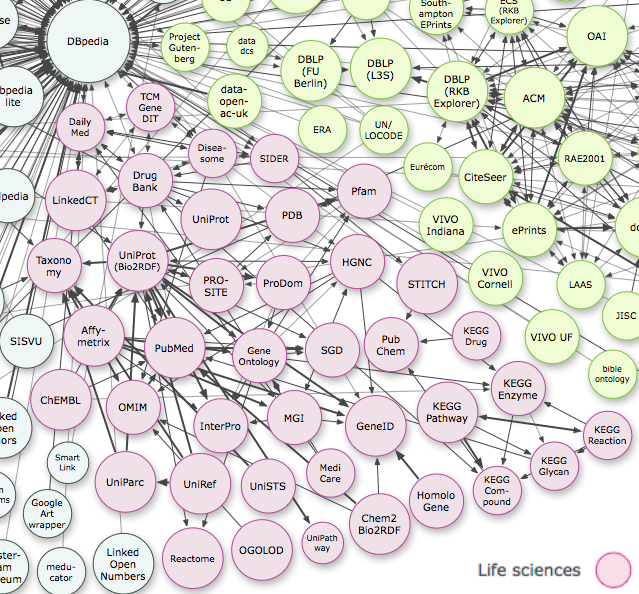
\includegraphics[width=1.0\columnwidth]{images/lod_cloud.png}
	\caption{Available datasets related to life sciences and pharmaceutical research.}
	\label{fig:lod}
\end{figure}

\subsection{Linked Open Drug Data (LODD)}
Particularly in the areas of health care and life sciences with the wealth of available data, large scale integration projects like Bio2RDF~\cite{bio2rdf}, Chem2Bio2RDF~\cite{chembio}, and the W3C HCLS’s (Health Care and Life Sciences) Linked Open Drug Data (LODD)\cite{lodd} have not only significantly contributed to the development of the Linked Open Data effort, but have also made social and technical contributions towards data integration, knowledge management, and knowledge discovery.

There are already many interesting information on pharmaceutical research available on the Web.
The sources of data range from drugs general information, interactions and impacts of the drugs on gene expression, through to the results of clinical trials.
LODD\cite{lodrug} has surveyed publicly available data about drugs, created Linked Data representations of the data sets, and identified interesting scientific and business questions that can be answered once the data sets are connected (cf. \autoref{fig:lod}).

\subsection{LODD Applications in Medical Domain}

There exists few approaches that address the medical and pharmaceutical applications using LODD.
\emph{TripleMap}\footnote{\url{http://www.triplemap.com}} is a project connecting widespread distribution of journal articles, patents and numerous databases in pharmaceutics research.
TripleMap as a web-based application provides a dynamic visual interface to integrate RDF datasets such as the LODD.
Showing an unexpected associations between entities related to researcher's interest is main advantage of TripleMap inspired  by the broad interconnected data available in the LODD data sets.
The goal of the TripleMap project is to deliver and sustain an ‘open pharmacological space’ by using and enhancing the state-of-the-art semantic web standards and technologies\cite{TripleMap}.

 Another related project is the Open Pharmacological Space (OPS), \emph{Open PHACTS} (Pharmacological Concept Triple Store) \footnote{\url{http://www.openphacts.org}} project under the European Innovative Medicines Initiative (IMI) \footnote{\url{http://www.imi.europa.eu/}}.
 The goal of this project is integration of chemical and biological data using Linked Data standards to support drug discovery~\cite{Openphacts}.

\emph{Linked Cancer Genome Atlas Database}\cite{SAL13} as another Linked Data project aims to create an atlas of genetic mutations responsible for cancer.
The project provides an infrastructure for making the cancer related data publicly accessible and to enable cancer researchers anywhere around the world to make and validate important discoveries.

Although these projects address the backend side of creating LODD applications, there has been a clear lack of applications with user-friendly, efficient and effective interfaces to make Linked Data resources accessible to end-users outside the biomedical community.
One of the use cases of LODD datasets addressed in this paper is authoring of \emph{Semantic Prescriptions} which are prescriptions enriched by Linked Open Data.

\section{Semantic Content Authoring}
\label{sec:sca}

A \emph{Semantic Document} is an intelligent document (with explicit semantic structure) which ``knows about" its own content so that it can be automatically processed in unforeseen ways.
Semantic documents facilitate a number of important aspects of information management~\cite{rdface}.
For \emph{search and retrieval}, they provide more efficient and effective search interfaces, such as faceted search~\cite{tunkenlang2009faceted} or question answering~\cite{Lopez2011}.
In \emph{information presentation}, they support more sophisticated ways of flexibly visualizing information, such as by means of semantic overlays as described in~\cite{Burel2009}.
In \emph{information integration}, they provide unified views on heterogeneous data stored in different applications by creating composite applications such as semantic mashups~\cite{Ankolekar2007}.
For \emph{personalization}, they provide customized and context-specific information which better fits user needs and will
result in delivering customized applications such as personalized semantic portals~\cite{ecs2007}.
For \emph{reusability} and \emph{interoperability}, they facilitate exchanging content between disparate systems and enabling applications such as executable papers~\cite{Muller2011}.


The above benefits, however, come at the cost of increased authoring effort. %~\cite{hasida2007,uren2006}
A \emph{Semantic Authoring User Interface} is a human accessible interface with capabilities for writing and modifying semantic documents which are either.
\emph{Semantic Content Authoring} (SCA) is a tool-supported manual composition process aiming at the creation of semantic documents which are either:
\begin{itemize}
	\item fully semantic in the sense that their original data model uses a semantic knowledge representation formalism (such as RDF, RDF-Schema or OWL) or
	\item based on a non-semantic representation form (e.g. text or hypertext), which is enriched with semantic representations during the authoring process.\\
\end{itemize}

With an ontology and a user interface appropriate for the type of content, semantic authoring can be easier than traditional composition of content and the resulting content can be of higher quality~\cite{hasida2007}.


\section{WYSIWYM User Interface}
\label{sec:wysiwym}

The term \emph{WYSIWYG} as an acronym for What-You-See-Is-What-You-Get is used in computing to describe a system in which content (text and graphics) displayed on-screen during editing appears in a form closely corresponding to its appearance when printed or displayed as a finished product.
WYSIWYG text authoring is meanwhile ubiquitous on the Web and part of most content creation and management workflows.
It is part of content management cystems (CMS), weblogs, wikis, fora, product data management systems and online shops, just to mention a few.
However, the WYSIWYG model has been criticized, primarily for the verbosity, poor support of semantics and low quality of the generated code and there have been voices advocating a change towards a \emph{WYSIWYM} (What-You-See-Is-What-You-Mean) model~\cite{Spiesser2004,Sauer2006}.

Similar to the WYSIWYG UI, the WYSIWYM term as defined in \cite{khaliliWISE2013} targets the novel aspect of integrated visualization, exploration and authoring of unstructured and semantic content.
The rationale of our WYSIWYM concept is to enrich the existing WYSIWYG presentational view of the content with UI components revealing the \emph{semantics} embedded in the content and enable the exploration and authoring of semantic content.
Instead of separating presentation, content and meaning, our WYSIWYM approach aims to integrate these aspects to facilitate the process of \emph{Semantic Content Authoring}.

\section{Semantic E-Prescribing}
\label{sec:sep}

E-health has evolved and emerged recently in many forms.
E-prescription is one of those forms and defined as a computer-generated prescription utilized by health-care providers.
E-prescribing as it is commonly called, is the use of an automated data entry system to generate a prescription that is then transmitted through a special network to a pharmacy in such a way that the data goes directly into the pharmacy’s computer system.
It plays an important role in improving the quality of patient care.
For the prescriber, e-prescribing happens when a physician uses a computer or handheld device with a software that allows him or her to (with the patient’s consent) electronically access information regarding a patient’s drug benefit coverage and medication history; electronically transmit the prescription to the patient’s pharmacy of choice; and, when the patient runs out of refills, his or her pharmacist can also electronically send a renewal request to the physician’s office for approval.

One of the main challenges of the current e-prescription systems is the heterogeneity and evolving nature of available information sources.
There exist already different sources of information addressing different aspects of pharmaceutical research.
Recruiting available e-prescription systems in order to connect the existing dynamic pharmaceutical information is a challenging task.
Linked Open Data when combined with existing e-prescribing systems, proposes a solution to tackle this challenge.

\begin{figure}[tb]
	\centering
		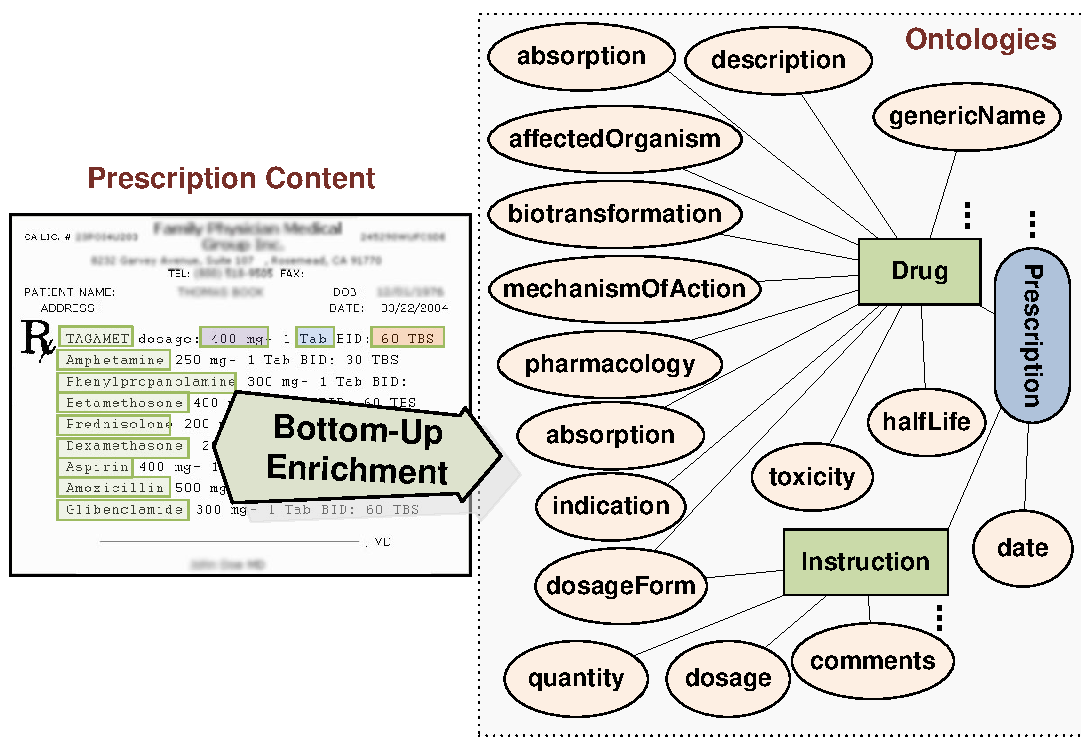
\includegraphics[width=1.0\columnwidth]{images/approaches.pdf}
	\caption{Bottom-up semantic enrichment of prescriptions.}
	\label{fig:botup}
\end{figure}

We define \emph{Semantic Medical Prescriptions} as intelligent e-prescription documents enriched by dynamic drug-related meta-data thereby know about their content and the possible interactions.
As depicted in \autoref{fig:botup}, semantic prescriptions are created based on a bottom-up process~\cite{khalili2012} in which normal e-prescriptions (unstructured or semi-structured with lower level of expressiveness) are enriched with semantic metadata coming from a set of predefined ontologies (with upper level of expressiveness).

\subsection{Architecture}

The Pharmer system architecture is depicted in \autoref{fig:arch} and consists of three layers:

\begin{figure}[tb]
	\centering
		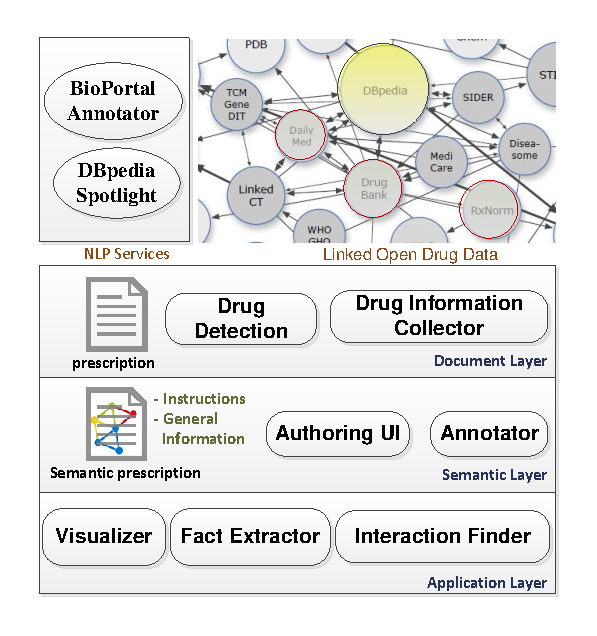
\includegraphics[width=1\columnwidth]{images/architecture.pdf}
	\caption{Architecture of the Pharmer system.}
	\label{fig:arch}
\end{figure}

\paragraph{Document Layer} This layer includes the traditional e-prescription document plus two components as \emph{Drug Detection} and \emph{Drug Information Collector}.
Drug detection component performs the natural language processing (NLP) of the e-prescription document to detect the terms referring to a drug in the prescription.
The component uses \emph{DBpedia Spotlight}~\cite{dbspotlight} and \emph{BioPortal annotator}~\cite{bioportal} NLP services to parse and analyze the text looking for known drugs.
DBpedia Spotlight is a tool for automatically annotating mentions of DBpedia resources in text (i.e. Named Entity Recognition).
BioPortal annotator is an ontology-based Web service that annotates public datasets with biomedical ontology concepts based on their textual metadata.
%describing NLP APIs

Automatic drug detection component is configurable so that users can easily add other existing NLP services for drug detection.
When user is writing the prescription, this component asynchronously performs the drug recognition and adds the related annotations as real-time semantic tagging.

Another component in this layer is drug information collector which grabs all the information regarding a specific drug from Linked Open Data.
To pursue this, it utilizes datasets such as DrugBank, DailyMed and RxNorm (available at \cite{lodd}) by sending federated SPARQL queries.

\paragraph{Semantic Layer}
There are two main components in this layer namely \emph{Annotator} and \emph{Authoring UI}.
The \emph{annotator} component handles the automatic annotation and embeds the general information of the drugs as meta-data into the e-prescription.
Annotator adopts the RDFa format. \emph{RDFa} (Resource Description Framework in attributes) is a W3C Recommendation that adds a set of attribute level extensions to XHTML for embedding RDF metadata within web documents.
RDFa fulfills the principles of interoperable metadata such as publisher independence, data reuse, self containment, schema modularity and evolvability.

The \emph{authoring UI} component provides users with a set of input forms to manually embed the meta-data related to prescription instructions into the prescription document.

\paragraph{Application Layer}
This layer provides a set of applications on top of the generated semantic prescriptions.
\emph{Interaction Finder} checks the possible interactions between the prescribed drugs and warn the prescriber about them.
\emph{Visualizer} is responsible for graphically representing the embedded semantics of a prescription (e.g. as depicted in \autoref{fig:graphview}).
The \emph{Fact Extractor} generates the RDF/Turtle representation of the semantic prescriptions.

\subsection{Features}
The main features of Pharmer can be summarized as:
\begin{itemize}
    \item \emph{WYSIWYM User Interface}.
    Pharmer employs the WYSIWYM (What-You-See-Is-What-You-Mean) concept for integrated visualization, exploration and authoring of un-structured and semantic content.
    In Pharmer, users are able to directly manipulate the conventional e-prescriptions in order to enrich them with semantics.
    The generated annotations can be viewed by different sets of user interfaces with are configurable by users.
    For example, users can select specific border/background colors to distinguish the annotated drugs in a prescription.
	\item \emph{Providing Different Semantic Views}.
	Semantic views allow the generation of different views on the same metadata schema and aggregations of the knowledge base based on the roles, personal preferences, and local policies of the intended users.
	Pharmer suggests two types of views: generic and domain specific views.
	Generic views provide visual representations of drug information (e.g. as information view depicted in \autoref{fig:screenshot} or graph view in \autoref{fig:graphview}).
	Domain specific views address the requirements of a particular domain user (e.g. a researcher need specific views for visualizing the atomic structure of chemical compounds).
	\item \emph{Real-time Drug Tagging.}
	Real-time tagging means creating drug annotations while the user is typing.
	This will significantly increase the annotation speed~\cite{OCA}.
	Users are not distracted since they do not have to interrupt their current authoring task.
	Pharmer has a client-side component which interacts with the server asynchronously to make real-time tagging possible.
	\item \emph{Drug Suggestion.}
		When searching for a drug, Pharmer suggests the similar drugs by taking into account the history of search terms.
    \item \emph{Automatic Drug Annotation.}
    Automatic annotation means the provision of facilities for automatic mark-up of prescriptions.
    The automatic process of annotating in Pharmer is composed basically of finding drug terms in prescription using an NLP service, mapping them against an ontology, and disambiguating common terms.
\end{itemize}



\begin{figure}[tb]
	\centering
		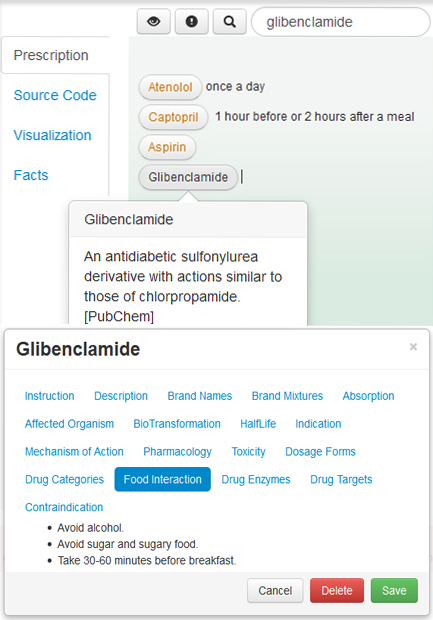
\includegraphics[width=0.95\columnwidth]{images/screenshot.jpg}
	\caption{Screenshot of the Pharmer application (general view, drug information view and prescription authoring view).}
	\label{fig:screenshot}
\end{figure}

\begin{figure}[tb]
	\centering
		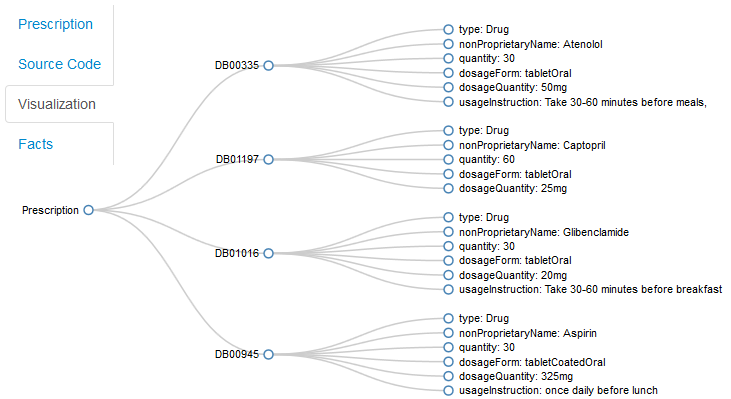
\includegraphics[width=1\columnwidth]{images/sc2.png}
	\caption{Graph view in Pharmer.}
	\label{fig:graphview}
\end{figure}

\section{Use cases}
\label{sec:usecases}

\subsection{Pharmer as a Ubiquitous Computing Platform for Semantic E-Prescribing}
\label{sec:mobile}

\begin{figure*}[tb]
 \centering
 \includegraphics[width=1.5\columnwidth]{images/sc_Pharmer.png}
	\caption{Screenshot of Pharmer Mobile Application (available at \url{http://bitili.com/Pharmer/mobile}).}
 \label{fig:mobile}
\end{figure*}

Mobile and ubiquitous computing devices are increasingly present and prevalent in the health contexts.
This trend brings a number of possibilities of \emph{mobile health} (m-health) to address critical aspects of health care and health system needs, by virtue of these devices’ ubiquity, simplicity, and cost-efficiency~\cite{mHealth}.
In particular, in the process of semantic e-prescribing, having a mobile application will facilitate the creation of semantic medical prescriptions using any device and in any location.

Pharmer mobile application as shown in \autoref{fig:mobile} provides a mobile user interface for authoring of semantic prescriptions as well as accessing multi-dimensional data on medical prescriptions.
Current ubiquitous devices are programmable and come with a growing set of facilities including multi-touch screens and cheap powerful embedded sensors, such as an accelerometer, digital compass, gyroscope, GPS, microphone, camera and other type of sensors.
Utilizing these rich set of facilities in the context of medical prescriptions will enrich the patient medical prescription with sensor data thereby improves the quality of e-health services.

\subsection{Pharmer as a Professional Social Network for Health-care Service Providers}
\label{sec:Pharmernet}
Pharmer offers couple of advantages over current e-prescribing systems:
The main benefit of using semantic prescriptions is the persistent connection to up-to-date drug information coming from multiple dynamic data sources.
So, when the information about a drug is updated occurs (e.g. change in its effects or interactions), the semantic prescription automatically adopts to this new change.

Once writing a prescription it is very critical to consider drug interactions.
Drug interactions are divided to three categories namely \emph{food-drug}, \emph{drug-drug} and \emph{drug-plant} interactions.
Coadministration can either be synergistic or antagonistic which respectively increase or decrease the drugs effect.
The interactions may sometimes lead to change in the drug effect.
By applying semantic prescriptions, all types of drug interactions are prevented and the probability of errors in prescriptions are reduced to a great extend.

A semantic prescription is a self-contained document which is aware of its content and is connected to the linked open data.
In contrast to database-oriented e-prescriptions, semantic prescriptions can easily be exchanged among other e-health systems without need to changing their related infrastructure hence enabling a connection between physicians, pharmacists, patients, pharmaceutical researchers, insurance and drug companies.

Pharmer as a prescribing tool is able to be incorporated in a health care social network.
Such a network composed of health care professionals and patients who collaboratively write, correct and modify prescriptions in a semantically enriched environment.
This social health care network provides patients and health care providers with services.
It further facilitates relations between patients and health care professionals in order to improve shared decision making (SDM).

As information source, the network accesses LODD, where diagnostic and prescribing data has been located as well.
Accessing such pieces of information, Pharmer is able to be used as a tool for diagnosis and prescribing in assistance to physicians.
Privacy of that network is also a critical point worth considerations.

\subsubsection{Shared Decision Making}
\label{subsec: SDM}
 The traditional model of medical decision-making, in which doctors make decisions on treatment has no longer used in updated health care.
 The role of the patient, instead, in the consultation has been highlighted, mainly through introducing‘patient-centred’ strategies.
 Therefor, nowadays the models promoting patients active involvement in the decision-making procedure becoming developed.
 
 A model introduced by Charles et al. defines shared decision making only under the following four key characteristics.
 These keys are:
 \begin{enumerate}
   \item both the patient and the doctor are involved
   \item both parties share information
   \item both parties take steps to build a consensus about the preferred treatment
   \item an agreement is reached on the treatment to implement
 \end{enumerate}

Pharmer as social network facilitates shared decision making through the connection amongst patient and physician on one hand and pharmacist on the other hand. According to Charles et al. model, Pharmer not only connects patients and physicians but also pharmacist as third party has an supervisory role on medication choice.

\subsubsection{Fast Diagnostic Tool}

Free access to LODD enables Pharmer to not only linked to e-prescribing systems but also to further assist physicians in diagnosis and treatment. Pharmer with direct connection to up-to-date information enables physicians to reconfirm their diagnosis and help them in finding proper treatment approaches.
Physician, after general examination, enters the observed symptoms in Pharmer system and there, with the wealth of data available, Pharmer assists in diagnosis followed by therapies.

\subsubsection{Privacy}
 Systems containing patient treatment history profiles, such as Pharmer, are required to be considered about privacy issues.
 This issue is solved by providing different users, with different views which is password protected.
 In such a protection, patient has only access to his profile while physician has access to all data of his patients, the same holds true for pharmacists and insurance companies.
 Other organisations(e.g. research institutes or pharma companies) can access to patients information as statistical data and only if the patient agrees.
 This protection helps Pharmer users to ensure data privacy.

\subsection{Example Scenario}
\label{sec:example}


\section{Conclusion}
\label{sec:conclusion}

Providing a consistent connection between patients, physicians, pharmacists, pharmaceutical researchers and pharma companies is a crucial step towards enhancing the quality of knowledge management and thereby e-health services in the pharmaceutical domain.
With Pharmer, we presented in this article an approach for user-friendly implementation of \emph{Semantic Prescriptions} as intelligent medical prescriptions to improve the integration and interoperability of e-prescribing systems with other e-health services.

We see the work presented in this article as an initial step in a larger research agenda aiming at promoting the authoring and annotation of semantically enriched medical documents.
Regarding future work, we envision to extend the Pharmer application towards different modalities, such that the annotation of images and other medical objects is supported.
Furthermore, we aim to integrate the other existing linked open datasets (e.g. related to publications, laboratories or insurance documents) into the Pharmer to extend its stakeholders.

\section*{Acknowledgments}
We would like to thank our colleagues from the AKSW research group (\url{http://aksw.org}) for their helpful comments and inspiring discussions during the development of the WYSIWYM model for authoring of semantic medical prescriptions.
This work was partially supported by a grant from the German Academic Exchange Service (DAAD).

\begin{spacing}{0.3}
\bibliographystyle{IEEEtran}
\bibliography{refs1,refs2,refs3}
\end{spacing}

% that's all folks
\end{document}


